\documentclass{standalone}
\usepackage{tikz}
\usetikzlibrary{positioning, arrows.meta, fit, backgrounds}

% Styles
\tikzstyle{io} = [rectangle, draw, minimum width=3.5cm, minimum height=1cm, fill=gray!20, font=\small]
\tikzstyle{block} = [rectangle, draw, minimum width=3cm, minimum height=1.5cm, fill=blue!10, font=\small, align=center]
\tikzstyle{bottleneck} = [rectangle, draw, minimum width=3cm, minimum height=1.4cm, fill=purple!15, font=\small]
\tikzstyle{sectionbox} = [draw=black, thick, dashed, inner sep=0.3cm, rounded corners=4pt]

\tikzstyle{arrow} = [thick, ->, >=stealth]
\tikzstyle{skip} = [arrow, dotted]
\tikzstyle{extraction} = [arrow, dashed, gray, bend right=30]

\begin{document}
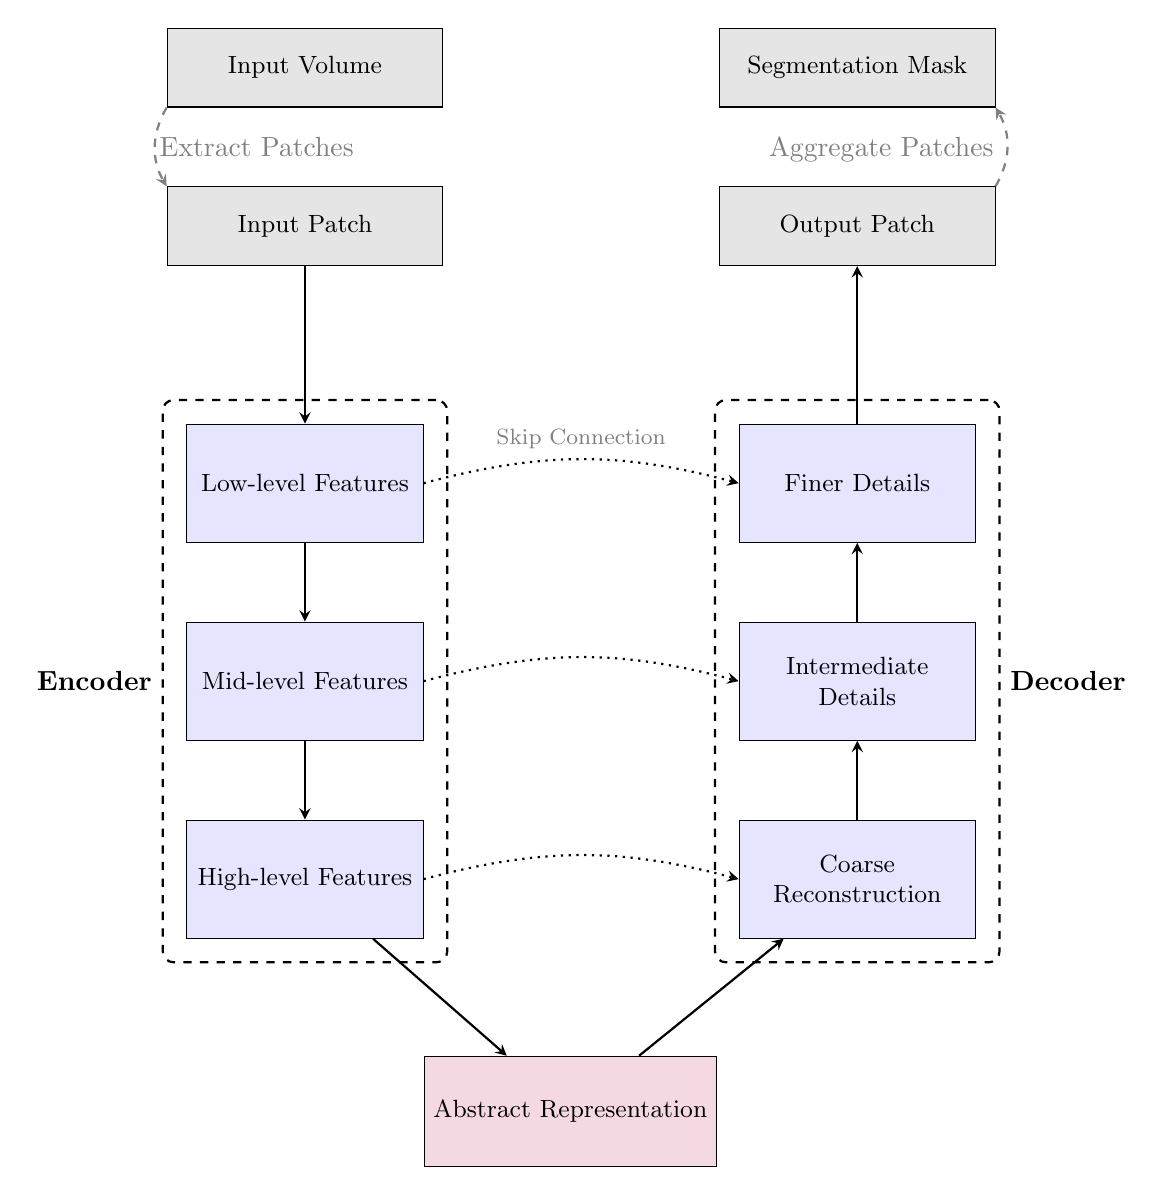
\begin{tikzpicture}[node distance=1.5cm and 3cm]

  % Input & output (left side)
  \node (input_img) [io] {Input Volume};
  \node (extract_patch) [below left=0.25cm and -2.5cm of input_img, text=gray, minimum width=1cm, align=left] {Extract Patches};
  \node (input_patch) [io, below=1cm of input_img] {Input Patch};

  % Encoder (left column)
  \node (enc1) [block, below=2cm of input_patch] {Low-level Features};
  \node (enc2) [block, below=1cm of enc1] {Mid-level Features};
  \node (enc3) [block, below=1cm of enc2] {High-level Features};

  % Bottleneck (centered)
  \node (bottleneck) [bottleneck, below right=4cm and 0cm of enc2.south east] {Abstract Representation};

  % Decoder (right column, mirrored)
  \node (dec1) [block, right=4cm of enc1] {Finer Details};
  \node (dec2) [block, right=4cm of enc2] {Intermediate\\ Details};
  \node (dec3) [block, right=4cm of enc3] {Coarse\\ Reconstruction};

  % Output
  \node (output_patch) [io, above=2cm of dec1] {Output Patch};
  \node (output_img) [io, above=1cm of output_patch] {Segmentation Mask};
  \node (extract_patch) [below right=0.25cm and -3cm of output_img, text=gray] {Aggregate Patches};

  % Arrows - main flow
  \draw[arrow] (input_patch) -- (enc1);
  \draw[arrow] (enc1) -- (enc2);
  \draw[arrow] (enc2) -- (enc3);
  \draw[arrow] (enc3) -- (bottleneck);
  \draw[arrow] (bottleneck) -- (dec3);
  \draw[arrow] (dec3) -- (dec2);
  \draw[arrow] (dec2) -- (dec1);
  \draw[arrow] (dec1) -- (output_patch);

  \draw[extraction] (input_img.south west) to (input_patch.north west);
  \draw[extraction] (output_patch.north east) to (output_img.south east);

  % Skip connections with labels
  \draw[skip] (enc3.east) to[bend left=15] node[midway, above, font=\footnotesize, gray] {} (dec3.west);
  \draw[skip] (enc2.east) to[bend left=15] node[midway, above, font=\footnotesize, gray] {} (dec2.west);
  \draw[skip] (enc1.east) to[bend left=15] node[midway, above, font=\footnotesize, gray] {Skip Connection} (dec1.west);

  % Section boxes
  \begin{scope}[on background layer]
    \node [sectionbox, fit=(enc1)(enc2)(enc3), label=left:\textbf{Encoder}] {};
    \node [sectionbox, fit=(dec1)(dec2)(dec3), label=right:\textbf{Decoder}] {};
  \end{scope}

\end{tikzpicture}
\end{document}
